\documentclass[UTF8,12pt]{article} % 12pt 为字号大小
\usepackage{amssymb,amsfonts,amsthm}
%\usepackage{fontspec,xltxtra,xunicode}
%\usepackage{times}
\usepackage{amsmath,bm}
\allowdisplaybreaks[4]
\usepackage{mdwlist}
\usepackage[colorlinks,linkcolor=blue]{hyperref}
\usepackage{cleveref}
\usepackage{float}
\usepackage{enumerate}
\usepackage{extarrows}
\numberwithin{equation}{section}

%----------
% 定义中文环境
%----------

\usepackage{xeCJK}
\setCJKmainfont[BoldFont={Heiti SC Light},ItalicFont={Kaiti SC Regular}]{Songti SC Regular}
\setCJKsansfont{Heiti SC Light}
\setCJKfamilyfont{song}{Songti SC Regular}
\setCJKfamilyfont{zhhei}{Heiti SC Light}
\setCJKfamilyfont{zhkai}{Kaiti SC Regular}
\setCJKfamilyfont{zhfs}{STFangsong}
\setCJKfamilyfont{zhli}{Libian SC Regular}
\setCJKfamilyfont{zhyou}{Yuanti SC Regular}

\newcommand*{\songti}{\CJKfamily{zhsong}} % 宋体
\newcommand*{\heiti}{\CJKfamily{zhhei}}   % 黑体
\newcommand*{\kaiti}{\CJKfamily{zhkai}}  % 楷体
\newcommand*{\fangsong}{\CJKfamily{zhfs}} % 仿宋
\newcommand*{\lishu}{\CJKfamily{zhli}}    % 隶书
\newcommand*{\yuanti}{\CJKfamily{zhyou}} % 圆体

%----------
% 版面设置
%----------
%首段缩进
\usepackage{indentfirst}
\setlength{\parindent}{2em}

%行距
\renewcommand{\baselinestretch}{1.2} % 1.2倍行距

%页边距
\usepackage[a4paper]{geometry}
\geometry{verbose,
  tmargin=2cm,% 上边距
  bmargin=2cm,% 下边距
  lmargin=2.5cm,% 左边距
  rmargin=2.5cm % 右边距
}


%----------
% 其他宏包
%----------
%图形相关
\usepackage[x11names]{xcolor} % must before tikz, x11names defines RoyalBlue3
\usepackage{graphicx}
\graphicspath{{figures/}}
\usepackage{pstricks,pst-plot,pst-eps}
\usepackage{subfig}
\def\pgfsysdriver{pgfsys-dvipdfmx.def} % put before tikz
\usepackage{tikz}

%原文照排
\usepackage{verbatim}

%网址
\usepackage{url}

%----------
% 定理、习题与解答环境
%----------
%定理环境
\usepackage[most]{tcolorbox}
\newtcbtheorem[number within=section]{theorem}{Theorem}{
     enhanced,
     breakable,
     sharp corners,
     attach boxed title to top left={
       yshifttext=-1mm
     },
     colback=blue!4!white,
     colframe=blue!75!black,
     fonttitle=\bfseries,
     boxed title style={
       sharp corners,
       size=small,
       colback=blue!75!black,
       colframe=blue!75!black,
     } 
}{theorem}

\newtcbtheorem[number within=section]{definition}{Definition}{
     enhanced,
     breakable,
     sharp corners,
     attach boxed title to top left={
       yshifttext=-1mm
     },
     colback=blue!4!white,
     colframe=blue!75!black,
     fonttitle=\bfseries,
     boxed title style={
       sharp corners,
       size=small,
       colback=blue!75!black,
       colframe=blue!75!black,
     } 
}{definition}

\newtcbtheorem[number within=section]{corollary}{Corollary}{
     enhanced,
     breakable,
     sharp corners,
     attach boxed title to top left={
       yshifttext=-1mm
     },
     colback=blue!4!white,
     colframe=blue!75!black,
     fonttitle=\bfseries,
     boxed title style={
       sharp corners,
       size=small,
       colback=blue!75!black,
       colframe=blue!75!black,
     } 
}{corollary}

\newtcbtheorem[number within=section]{myboxes}{Box}{
     enhanced,
     breakable,
     sharp corners,
     attach boxed title to top left={
       yshifttext=-1mm
     },
     %colback=white,
     colframe=black!75!white,
     fonttitle=\bfseries,
     boxed title style={
       sharp corners,
       size=small,
       colback=black!75!white,
       colframe=black!75!white,
     } 
}{myboxes}

%习题环境
\newtcbtheorem[number within=section]{exercise}{Problem}{
     enhanced,
     breakable,
     sharp corners,
     attach boxed title to top left={
       yshifttext=-1mm
     },
     colback=white,
     colframe=black,
     fonttitle=\bfseries,
     boxed title style={
       sharp corners,
       size=small,
       colback=black,
       colframe=black,
     } 
}{Problem}

%解答环境
\ifx\proof\undefined\
\newenvironment{proof}[1][\protect\proofname]{\par
\normalfont\topsep6\p@\@plus6\p@\relax
\trivlist
\itemindent\parindent
\item[\hskip\labelsep
\scshape
#1]\ignorespaces
}{%
\endtrivlist\@endpefalse
}
\fi

\renewcommand{\proofname}{\it{Solution}}

%==========
% 正文部分
%==========

\begin{document}

\title{Chapter 3: Angular Momentum}
\author{Yuquan Chen}
\date{2019/04/16} % 若不需要自动插入日期,则去掉前面的注释;{ } 中也可以自定义日期格式
\maketitle

We have discussed position and momentum operator before, now let's consider the rotation of a system, which leads to angular position and angular momentum. Before we dive in, there's some prerequisites we should know.

\section{Some prerequisites}

In a 3D system, we use $\vec{r} = (x,y,z)$ to represent the coordinate, and the momentum is $\vec{p} = (p_{x}, p_{y}, p_{z})$. In position representation, we have $p_{x} \leftrightarrow -i\hbar \frac{\partial}{\partial x}$, $p_{y} \leftrightarrow -i\hbar \frac{\partial}{\partial y}$, and $p_{z} \leftrightarrow -i\hbar \frac{\partial}{\partial z}$, together we get $\vec{p} = (-i\hbar \frac{\partial}{\partial x}, -i\hbar \frac{\partial}{\partial y}, -i\hbar \frac{\partial}{\partial z}) = -i\hbar \vec{\nabla}$.

Now let's switch to spherical coordinate $(r, \theta, \varphi)$.
\begin{figure}[H]
\begin{center}
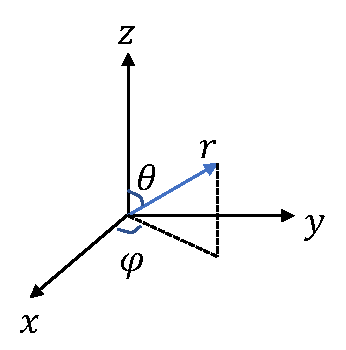
\includegraphics[width=4cm]{sph}
%\caption{}
%\label{}
\end{center}
\end{figure}

For a point in space, we use a ket $|\psi\rangle$ to represent it,
\begin{align}
\begin{cases}x = r\sin\theta\cos\varphi \\ y = r\sin\theta\sin\varphi \\ z = r\cos\theta\end{cases} \Rightarrow r = \sqrt{x^{2} + y^{2} +z^{2}}
\label{coordinate}
\end{align}
now let's consider a rotation along $\hat{z}$ direction. Here $\varphi$ becomes $\varphi + d\varphi$, and $r,\theta$ remain the same. We have 
\begin{align}
|x,y,z\rangle \xrightarrow{\text{rotation}} |x', y', z'\rangle
\end{align}
and the corresponding
\begin{align}
(r,\theta,\varphi) \xrightarrow{\text{rotation}} (r, \theta, \varphi + d\varphi)
\end{align}
then we try to find out the expression of $x',y',z'$ in terms of $r,\theta,\varphi, d\varphi$
\begin{align}
\begin{cases}
x' = r\sin\theta\cos(\varphi+d\varphi) \simeq r\sin\theta\cos\varphi - r\sin\theta\sin\varphi d\varphi \\
y' = r\sin\theta\sin(\varphi+d\varphi) \simeq  r\sin\theta\sin\varphi + r\sin\theta\cos\varphi d\varphi \\
z' = r\cos\theta = z
\end{cases}
\Rightarrow \begin{cases}
x' = x - yd\varphi\\
y' = y + xd\varphi\\
z' = z
\end{cases}
\end{align}

On a spin-$\frac{1}{2}$ system, we have Pauli operators $\sigma_{x}, \sigma_{y}, \sigma_{z}$. In the $\sigma_{z}$ basis, we have
\begin{align}
\sigma_{x} = \begin{pmatrix}0&1\\1&0\end{pmatrix}, \sigma_{y} = \begin{pmatrix}0&-i\\i&0\end{pmatrix}, \sigma_{z} = \begin{pmatrix}1&0\\0&-1\end{pmatrix}
\end{align}
and
\begin{align}
[\sigma_{k}, \sigma_{l}] = 2i\varepsilon_{klm}\sigma_{m}, ~~\varepsilon_{klm} = \begin{cases}1 &\text{if } k,l,m \text{ in order}\\-1 &\text{if out of order}\end{cases}
\end{align}
define the spin operator,
\begin{align}
\begin{cases}
\vec{S} = \frac{\hbar}{2}\vec{\sigma},~ S_{z} = \frac{\hbar}{2}\sigma_{z}\\
\vec{\sigma} = (\sigma_{x}, \sigma_{y}, \sigma_{z})
\end{cases}
\end{align}
here we should mention that $\boxed{[S_{k}, S_{l}] = i\hbar\varepsilon_{klm}S_{m}}$ is generally true for angular momentum operators, including spin-$\frac{1}{2}$ operators.

\begin{align}
\vec{S}^{2} = S_{x}^{2} + S_{y}^{2} + S_{z}^{2} = \frac{\hbar^{2}}{4} \left(\sigma_{x}^{2} + \sigma_{y}^{2} + \sigma_{z}^{2}\right) = \frac{3}{4} \hbar^{2} I
\end{align}
notice that for each $k$ in $x, y, z$, we have $\boxed{\sigma_{k}^{2} = I}$ so $\vec{S}^{2} \propto I$, and we also have $\boxed{[\vec{S}^{2}, S_{k}] = 0}$. If we define unite length vector
\begin{align}
\vec{n} = (\sin\theta\cos\varphi, \sin\theta\sin\varphi, \cos\theta)
\end{align}
we have
\begin{align}
\vec{\sigma}\cdot\vec{n} = \sigma_{x}\sin\theta\cos\varphi + \sigma_{y}\sin\theta\sin\varphi + \sigma_{z}\cos\theta
\end{align}

Noticed that if you try to use Mathematica to implement $\vec{\sigma}\cdot\vec{n}$, use the expression $\vec{n}\cdot\vec{\sigma}$ instead. When we are dealing with matrix exponential, we use Taylor expansion
\begin{align}
e^{i\phi\hat{\sigma}_{x}} = I + i\phi \sigma_{x} - \frac{\phi^{2}\sigma_{x}^{2}}{2!} + \frac{i\phi^{3}\sigma_{x}^{3}}{3!} - ...
\end{align}
we use
\begin{align}
\begin{cases}
e^{\hat{A}} = I + \hat{A} + \frac{\hat{A}^{2}}{2!} + ... + \frac{\hat{A}^{n}}{n!} + ...\\
\sigma_{x}^{2} = I
\end{cases}
\end{align}
to get
\begin{align}
e^{i\phi\hat{\sigma}_{x}} &= \left(I - \frac{\phi^{2}}{2!}I + \frac{\phi^{4}}{4!}I - ...\right) + i\sigma_{x} \left(\phi - \frac{\phi^{3}}{3!} + \frac{\phi^{5}}{5!} - ...\right) \\
&= \cos\phi I + i\sin\phi\sigma_{x}
\end{align}

\section{Orbital angular momentum}

Let's consider a small rotation: $\varphi \rightarrow \varphi + d\varphi$,
\begin{align}
\begin{cases}
x' \simeq x - yd\varphi \\
y' \simeq y + xd\varphi \\
z' = z
\end{cases}
\end{align}
if we have a state $|\psi\rangle$ expressed in position coordinate $\langle x,y,z|\psi\rangle = \psi(x,y,z)$ (we can also write it in spherical basis $\psi(r,\theta,\varphi)$, as we discussed above), then we apply a rotation to the state, we get from
\begin{align}
\psi(r,\theta,\varphi) \rightarrow \psi(r,\theta,\varphi - d\varphi)
\end{align}
and we know
\begin{align}
\psi(r,\theta,\varphi - d\varphi) \simeq \psi(r,\theta,\varphi) - d\varphi \cdot \frac{\partial}{\partial \varphi} \psi(r,\theta,\varphi)
\end{align}
we can express this small rotation as
\begin{align}
I - \frac{\partial}{\partial\varphi} = I + \frac{1}{i\hbar}\hat{L}_{z}
\end{align}
here we can see the relationship:
\begin{align}
\hat{L}_{z} \xlongequal{\varphi\text{ coordinate}} -i\hbar\frac{\partial}{\partial\varphi} \longleftrightarrow p_{x} \xlongequal{x\text{ coordinate}} -i\hbar\frac{\partial}{\partial x}
\end{align}
then we express $\hat{L}_{z}$ in $x,y,z$ coordinates,
\begin{align}
\psi(x,y,z) \xrightarrow{I - \frac{\partial}{\partial \varphi}} \psi(x', y', z')
\end{align}
rotate axis along $z$ by $d\varphi$
\begin{align}
\begin{cases}
x' = x - yd\varphi \\
y' = y + xd\varphi \\
z' = z
\end{cases}
\xrightarrow{\text{want } -d\varphi}
\begin{cases}
x' = x + yd\varphi \\
y' = y - xd\varphi \\
z' = z
\end{cases}
\end{align}
so
\begin{align}
\psi(x', y', z') &\simeq \psi(x + yd\varphi, y - xd\varphi,z) \\
&= \psi(x,y,z) + yd\varphi\frac{\partial}{\partial x}\psi(x,y,z) - xd\varphi\frac{\partial}{\partial y}\psi(x,y,z)
\end{align}
we have
\begin{align}
p_{x} \leftrightarrow -i\hbar\frac{\partial}{\partial x},~ p_{y} \leftrightarrow -i\hbar\frac{\partial}{\partial y}
\end{align}
so
\begin{align}
\psi(x', y', z') &= \psi(x,y,z) + yd\varphi\left(\frac{\hat{p}_{x}}{-i\hbar}\right)\psi(x,y,z) - xd\varphi\left(\frac{\hat{p}_{y}}{-i\hbar}\right)\psi(x,y,z) \\
&= \left(I + \frac{1}{-i\hbar}d\varphi(yp_{x} - xp_{y})\right) \psi(x,y,z) \\
&= \left(I + \frac{1}{i\hbar}\hat{L}_{z}\right) \psi(x,y,z)
\end{align}

So $\hat{L}_{z}$ expressed with $x,y,z$ coordinate with respected operators should be
\begin{align}
\hat{L}_{z} = \hat{x}\hat{p}_{y} - \hat{y}\hat{p}_{x}
\end{align}
similarly, we can write out the $\hat{L}_{x}$ and $\hat{L}_{y}$. In total,
\begin{align}
\boxed{\begin{cases}
\hat{L}_{x} = \hat{y}\hat{p}_{z} - \hat{z}\hat{p}_{y} \\
\hat{L}_{y} = \hat{z}\hat{p}_{x} - \hat{x}\hat{p}_{z} \\
\hat{L}_{z} = \hat{x}\hat{p}_{y} - \hat{y}\hat{p}_{x}
\end{cases}}
\end{align}
which is the same as classical mechanics $\vec{L} = \vec{r} \times \vec{p}$, so we get an orbital angular momentum operator in analog to classical. For now, we've already find out the $\hat{L}_{x}, \hat{L}_{y}, \hat{L}_{z}$ represented in $x,y,z$ coordinate. Let's try to write them in $r,\theta,\varphi$ coordinate. We can replace the $\hat{p}_{i}$ as $-i\hbar\frac{\partial}{\partial i}$, and use (\ref{coordinate}) to replace $x,y,z$ to $r,\theta,\varphi$.
\begin{align}
\begin{cases}
L_{x} = i\hbar\left(\sin\varphi\frac{\partial}{\partial\varphi} + \cot\theta\cos\varphi\frac{\partial}{\partial\varphi}\right) \\
L_{y} = i\hbar\left(-\cos\varphi\frac{\partial}{\partial\theta} + \cot\theta\sin\varphi\frac{\partial}{\partial\varphi}\right) \\
L_{z} = -i\hbar\frac{\partial}{\partial\varphi}
\end{cases}
\label{spherical}
\end{align}

After defined $L_{i}$ in both $x,y,z$ and $r,\theta, \varphi$ coordinates, we can now explore some properties of orbital angular momentum.
\begin{enumerate*}
\item $[L_{x}, L_{y}] = i\hbar L_{z}$
\begin{proof}[Proof]
We already know
\begin{align}
\begin{cases}
[x, p_{x}] = i\hbar \\
[x,y] = [x,p_{y}] = [p_{x}, p_{y}] = 0
\end{cases}
\end{align}
so
\begin{align}
[yp_{z} - zp_{y}, zp_{x} - xp_{z}] &= [yp_{z}, zp_{x}] + [yp_{z}, -xp_{z}] + [-zp_{y}, zp_{x}] + [-zp_{y}, -xp_{z}] \\
&= [yp_{z}, zp_{x}] + [-zp_{y}, -xp_{z}] \\
&= yp_{x}[p_{z},z] + p_{y}x[z,p_{z}] \\
&= i\hbar\left(xp_{y} - yp_{x}\right) = i\hbar L_{z}
\end{align}
\end{proof}
Furthermore, we can easily proof that 
\begin{align}
\boxed{[L_{k}, L_{l}] = i\hbar\varepsilon_{k,l,m}L_{m},~ \varepsilon_{klm} = \begin{cases}1&\text{if }k,l,m\text{ in order}\\-1&\text{if out of order}\end{cases}}
\end{align}
\item $\boxed{[L^{2}, L_{i}] = 0}$, which is similar to $[S^{2}, S_{i}] = 0$.
\begin{proof}[Proof]
We know that
$$L^{2} = L_{x}^{2} + L_{y}^{2} + L_{z}^{2},~ [A^{2},B] = A[A,B] + [A,B]A$$
so
\begin{align}
[L^{2}, L_{x}] &= [L_{x}^{2} + L_{y}^{2} + L_{z}^{2}, L_{x}] = [L_{y}^{2}, L_{x}] + [L_{z}^{2}, L_{x}] \\
&= L_{y}[L_{y}, L_{x}] + [L_{y}, L_{x}]L_{y} + L_{z}[L_{z}, L_{x}] + [L_{z}, L_{x}]L_{z} \\
&= -i\hbar L_{y}L_{z} -i\hbar L_{z}L_{y} + i\hbar L_{z}L_{y} + i\hbar L_{y}L_{z} \\
&= 0
\end{align}
\end{proof}
\end{enumerate*}
so in total,
\begin{myboxes}{Properties of orbital angular momentum}{}
\begin{enumerate*}
\item \begin{align*}
[L_{k}, L_{l}] = i\hbar\varepsilon_{k,l,m}L_{m},~ \varepsilon_{klm} = \begin{cases}1&\text{if }k,l,m\text{ in order}\\-1&\text{if out of order}\end{cases}
\end{align*}
\item $$[L^{2}, L_{i}] = 0$$
\end{enumerate*}
\end{myboxes}

Now let's consider the eigen equation with $L^{2}$ and $L_{z}$. Recall that if $\hat{A}, \hat{B}$ are Hermitian, and $[\hat{A}, \hat{B}] = 0$, then there exists $\{|\psi\rangle\}$ giving
$$\begin{cases}\hat{A}|\psi\rangle = a|\psi\rangle \\ \hat{B}|\psi\rangle = b|\psi\rangle\end{cases}$$
or we can say $\{|\psi\rangle\}$ is the mutual eigen state. Here we already have $[L^{2}, L_{z}] = 0$, let $|y\rangle$ to be one of these states, so
\begin{align}
\begin{cases}
L_{z}|y\rangle = m\hbar|y\rangle \\
L^{2}|y\rangle = \beta\hbar^{2}|y\rangle \\
\end{cases}
\end{align}
where $m,\beta$ are numbers. $|y\rangle$ needs to be normalized, $\langle y|y\rangle = 1$
\begin{align}
\beta\hbar^{2} = \langle y|L^{2}|y\rangle = \langle y|L_{x}^{2} + L_{y}^{2} + L_{z}^{2}|y\rangle \ge \langle y|L_{z}^{2}|y\rangle = m^{2}\hbar^{2}
\end{align}
so
\begin{align}
\beta \ge m^{2}
\end{align}
    in spherical coordinate, as above we can express $L^{2}, L_{z}$ all in just $\theta, \varphi$ without $r$. $L^{2}, L_{z}$ only relates to angular coordinates $\{\theta, \varphi\}$ as the angular representation. The eigen function for $L_{z}$ in coordinates $\{\theta, \varphi\}$ is $\langle\theta,\varphi|L_{z}|y\rangle = \lambda\langle\theta,\varphi|y\rangle$. To make the expression more convenient (we will know the reason soon), let's set $\lambda = m\hbar$.
\begin{align}
\langle\theta, \varphi|y\rangle &= y(\theta, \varphi) \\
\langle\theta,\varphi|L_{z}|y\rangle &= m\hbar\langle\theta,\varphi|y\rangle \\
&= -i\hbar\frac{\partial}{\partial\varphi}\langle\theta,\varphi|y\rangle
\end{align}
then we can solve the equation
\begin{align}
-i\hbar\frac{\partial}{\partial\varphi} y(\theta,\varphi) = m\hbar y(\theta,\varphi) \Rightarrow y(\theta,\varphi) \propto e^{im\varphi}
\label{Lz}
\end{align}
and $\varphi \rightarrow \varphi + 2\pi$ should give the same wave function, so we have
\begin{align}
e^{im\varphi} = e^{im(\varphi + 2\pi)} \Rightarrow e^{i2\pi m} = 1
\end{align}
so $m$ should be an integer, $m = 0, \pm1, \pm2, ...$, and now we know why we need to set $\lambda = m\hbar$ before. Further, we have the eigen function for $L^{2}$
\begin{align}
\langle\theta, \varphi|L^{2}|y\rangle = \beta\hbar^{2}\langle\theta,\varphi|y\rangle
\end{align}
notice that the original eigen function is $\langle\theta, \varphi|L^{2}|y\rangle = \lambda'\langle\theta,\varphi|y\rangle$, and the reason to let $\lambda' = \beta\hbar^{2}$ is similar to the former one, we will see it soon. By using (\ref{spherical}) to calculate $L^{2} = L_{x}^{2} + L_{y}^{2} + L_{z}^{2}$, we get
\begin{align}
&\Rightarrow L^{2} = -\hbar^{2}\left[\frac{1}{\sin\theta}\frac{\partial}{\partial\theta}\left(\sin\theta\frac{\partial}{\partial\theta}\right) + \frac{1}{\sin^{2}\theta}\frac{\partial^{2}}{\partial\varphi^{2}}\right] \\
&\Rightarrow -\left[\frac{1}{\sin\theta}\frac{\partial}{\partial\theta}\left(\sin\theta\frac{\partial}{\partial\theta}\right) + \frac{1}{\sin^{2}\theta}\frac{\partial^{2}}{\partial\varphi^{2}}\right] y(\theta,\varphi) = \beta y(\theta,\varphi)
\end{align}
use (\ref{Lz}) we can get $\frac{\partial^{2}}{\partial\varphi^{2}} y(\theta,\varphi) = -m^{2} y(\theta,\varphi)$,
\begin{align}
&\Rightarrow \left[\frac{1}{\sin\theta}\frac{\partial}{\partial\theta}\left(\sin\theta\frac{\partial}{\partial\theta}\right) + \frac{m^{2}}{\sin^{2}\theta} - \beta\right] y(\theta,\varphi) = 0
\end{align}

There's a solution proportional to a spherical function $P_{l}^{m}(\cos\theta)$ called associated Legendre polynomial. We need
\begin{align}
\begin{cases}
\beta = l(l+1),~ l = 0,1,2,... \\
m = -l, -l+1, ..., l-1, l
\end{cases}
\end{align}
the full solution is called Spherical Harmonics function
\begin{align}
Y_{lm} = y(\theta,\varphi) = \sqrt{\frac{(2l+1)(l-m)!}{4\pi(l+m)!}}P_{l}^{m}(\cos\theta) e^{im\varphi}
\end{align}
as a normalized solution, with $\begin{cases}l = 0,1,2,...\\m = -l, -l+1,..., l-1, l\end{cases}$ as quantum number (the solution $Y_{lm}$ needs two numbers to specify, just like an ID). As we discussed above, $Y_{lm}$ is normalized, which means
\begin{align}
\int_{0}^{2\pi} d\varphi \int_{0}^{\pi} \sin\theta Y_{l'm'}^{*} Y_{lm} d\theta = \delta_{ll'}\delta_{mm'} = \begin{cases}1&\text{if }l=l', m=m'\\0&\text{otherwise}\end{cases}
\end{align}

From $Y_{lm}$, we know $|y\rangle = |l,m\rangle$. $\{|l,m\rangle\}$ form a basis, which has $2l + 1$ dimension.

\section{General properties of angular momentum}

This section corresponds to section 3.5 of \textit{Sakurai}. Similar to $\vec{S}, \vec{L}$, we use $\vec{J}$ for general case, and the corresponding eigen state is $|j,m\rangle$, with
\begin{enumerate*}
\item $[J_{k}, J_{l}] = i\hbar\varepsilon_{klm}J_{m}$
\item $[J^{2}, J_{i}] = 0$
\item $J_{z}|j,m\rangle = m\hbar|j,m\rangle$
\item $J^{2}|j,m\rangle = \beta\hbar^{2}|j,m\rangle$
\end{enumerate*}
and we will proof $\beta = j(j + 1)$ soon. Define ladder operator $J_{+}, J_{-}$ as below
\begin{align}
\begin{cases}
J_{+} = J_{x} + iJ_{y} \\
J_{-} = J_{x} - iJ_{y}
\end{cases}
\end{align}
from the definition, we can get
\begin{align}
J_{-} &= J_{+}^{\dag} \\
[J_{z}, J_{+}] &= \hbar J_{+} \\
[J_{z}, J_{-}] &= -\hbar J_{-} \\
[J_{+}, J_{-}] &= 2\hbar J_{z} \\
J_{-}J_{+} &= J^{2} - J_{z}^{2} - \hbar J_{z} \\
J_{+}J_{-} &= J^{2} - J_{z}^{2} + \hbar J_{z}
\end{align}
with $J_{z}|j,m\rangle = m\hbar|j,m\rangle$, try to find some properties.
\begin{align}
J_{z}J_{+}|j,m\rangle = \left([J_{z}, J_{+}] + J_{+}J_{z}\right)|j,m\rangle = (\hbar J_{+} + J_{+}J_{z})|j,m\rangle = (m+1)\hbar J_{+}|j,m\rangle
\end{align}
Let $|\xi\rangle = J_{+}|j,m\rangle$, so there is $J_{z}|\xi\rangle = (m+1)\hbar|\xi\rangle$. We then know $|\xi\rangle$ has something to do with $|j,m+1\rangle$ (which means $J_{+}$ increases quantum state $|j,m\rangle$ by one unit), $J_{+}|j,m\rangle \rightarrow c|j,m+1\rangle$. Similarly, we have $J_{-}|j,m\rangle \rightarrow c'|j,m-1\rangle$, and we try to find out $c, c'$.
\begin{enumerate*}
\item Upper bound for $|j,m\rangle = |j,M_{\text{up}}\rangle$, $J_{+}|j,M_{\text{up}}\rangle = 0$
\begin{align}
0 &= J_{-}J_{+}|j,M_{\text{up}}\rangle = \left(J^{2} - J_{z}^{2} - \hbar J_{z}\right)|j,M_{\text{up}}\rangle \\
&= \left(\beta\hbar^{2} - M_{\text{up}}^{2}\hbar^{2} - M_{\text{up}}\hbar^{2}\right)|j,M_{\text{up}}\rangle \\
\Rightarrow \beta &= M_{\text{up}}(M_{\text{up}} + 1)
\end{align}
\item Lower bound of $|j,m\rangle = |j,M_{\text{low}}\rangle$, $J_{-}|j,M_{\text{low}}\rangle = 0$
\begin{align}
0 = J_{+}J_{-}|j,M_{\text{low}}\rangle \Rightarrow \beta = M_{\text{low}}(M_{\text{low}} - 1) 
\end{align}
\end{enumerate*}
if we have $j = M_{\text{up}} = -M_{\text{low}}$, then $\beta = j(j+1)$

\end{document}